\chapter{Metales de transición y complejos de coordinación}\label{ch:b2:coordination-complexes}

En 1893 un químico de veintiséis años, Alfred Werner, se propuso explicar un enigma.
El cloruro de cobalto(III) forma cuatro compuestos con el amoníaco, \ce{CoCl3.6NH3},
\ce{CoCl3.5NH3} y dos de fórmula \ce{CoCl3.4NH3}, uno verde y otro violeta.
El nitrato de plata precipita de inmediato los tres cloruros del primero, dos del
segundo y solo uno de cada uno de los dos últimos. La respuesta de Werner (seis
grupos sujetos alrededor del metal en los vértices de un octaedro, y el resto fuera)
fundó la química de la coordinación. Este capítulo extiende los complejos del
volumen del primer año a su geometría, sus isómeros, sus nombres y un recuento de
electrones que predice qué carbonilos metálicos existen.

\begin{recall}
El volumen del primer año: complejo, átomo central, ligando, ligando polidentado, quelato,
constantes de formación, número de coordinación; configuraciones electrónicas de los
iones de los metales de transición (los electrones $n$s se pierden primero); ácidos y bases de Lewis,
enlaces dativos; RPECV; números de oxidación; enantiómeros. \Cref{ch:b2:atomic-orbitals}:
los orbitales d y el orden de los niveles 4s y 3d.
\end{recall}

\begin{omfigure}
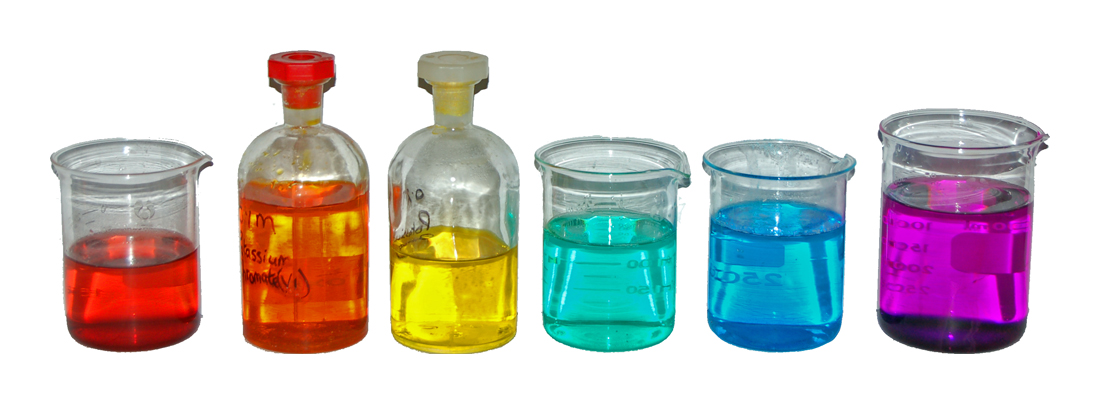
\includegraphics[width=0.8\linewidth]{images/book3/tm-solutions.jpg}

{\small Disoluciones acuosas de compuestos de metales de transición: de izquierda a derecha,
nitrato de cobalto(II), dicromato de potasio, cromato de potasio, cloruro de níquel(II),
sulfato de cobre(II) y permanganato de potasio. Los colores de las disoluciones de cobalto, níquel
y cobre proceden de sus acuocomplejos. (Fotografía: Benjah-bmm27,
dominio público, Wikimedia Commons.)}
\end{omfigure}

\section{El bloque d}

\begin{definition}[Elemento de transición]\label{def:b2:coordination-complexes:transition-element}
Un \emph{elemento de transición}\index{elemento de transicion@elemento de transición} es un elemento cuyo átomo, o
alguno de cuyos iones habituales, tiene una subcapa d parcialmente llena. Un ion de un elemento así
con $n$ electrones en sus orbitales d tiene una \emph{configuración $d^n$}\index{configuracion dn@configuración $d^n$}.
\end{definition}

\begin{proposition}[Recuento de los electrones d]\label{prop:b2:coordination-complexes:dn}
Un ion de metal de transición $\mathrm M^{m+}$ del grupo número $g$ (3 a 12) tiene una configuración $d^n$
con $n = g - m$.
\end{proposition}

\begin{proof}
El átomo neutro tiene $g$ electrones además de los del gas noble precedente, en los orbitales $n$s y
$(n - 1)$d. En los iones, los orbitales d están por debajo del orbital s
(\cref{ex:b2:atomic-orbitals:iron}): los $g - m$ electrones de valencia restantes son todos
electrones d.
\end{proof}

Por ejemplo, \ce{Fe^2+} (grupo 8) es $d^6$, \ce{Cu^2+} (grupo 11) $d^9$, \ce{Co^3+} (grupo 9)
$d^6$ y \ce{Pt^2+} (grupo 10) $d^8$.

\section{Ligandos}

\begin{definition}[Denticidad]\label{def:b2:coordination-complexes:denticity}
La \emph{denticidad}\index{denticidad} de un ligando es el número de sus átomos unidos al
mismo átomo central. Un \emph{ligando monodentado}\index{ligando monodentado} se une
por un átomo (\ce{H2O}, \ce{NH3}, \ce{Cl-}, \ce{CO}), y un \emph{ligando
bidentado}\index{ligando bidentado}, por dos (la etano-1,2-diamina, abreviada en; el
ion etanodioato, ox). Un \emph{ligando puente}\index{ligando puente} se une a dos
átomos metálicos a la vez. Un \emph{ligando ambidentado}\index{ligando ambidentado} puede unirse
por uno u otro de dos átomos distintos, como el ion nitrito (por N o por O) o el
tiocianato (por S o por N).
\end{definition}

\begin{definition}[Esfera de coordinación]\label{def:b2:coordination-complexes:coordination-sphere}
La \emph{esfera de coordinación}\index{esfera de coordinacion@esfera de coordinación} de un complejo es el conjunto formado por
el átomo central y los ligandos unidos a él, que se escribe entre corchetes; los iones
fuera de los corchetes son contraiones, no unidos al metal.
\end{definition}

\begin{omfigure}
\setchemfig{atom sep=2.2em}
\chemfig{M*5(-H_2N-CH_2-CH_2-NH_2-)}
\qquad
\chemfig{M*5(-O-(=O)-(=O)-O-)}
\qquad
\chemfig{N(-[:120]CH_2COO^{-})(-[:240]CH_2COO^{-})-CH_2-CH_2-N(-[:60]CH_2COO^{-})(-[:-60]CH_2COO^{-})}

\medskip
{\small Ligandos quelantes. A la izquierda: la etano-1,2-diamina (en), bidentada por sus dos
nitrógenos. En el centro: el ion etanodioato (ox), bidentado por dos oxígenos. A la derecha:
el anión edta, que envuelve un ion metálico con sus dos nitrógenos y sus cuatro
oxígenos carboxilato (hexadentado).}
\end{omfigure}

\section{Números de coordinación y geometrías}

Dos, cuatro y seis son los números de coordinación más frecuentes. La plata(I) y el oro(I) dan
complejos lineales (\ce{[Ag(NH3)2]+}); cuatro ligandos forman un tetraedro
(\ce{[CoCl4]^2-}, \ce{[Zn(NH3)4]^2+}) o un cuadrado (\ce{[PtCl4]^2-}, \ce{[Ni(CN)4]^2-});
cinco, una bipirámide trigonal (\ce{Fe(CO)5}); seis, con mucho los más frecuentes, un
octaedro.

\begin{omfigure}
\begin{tikzpicture}[font=\small]
  \node[omligand] at (-0.8,0) {}; \node[omligand] at (0.8,0) {};
  \draw[thick, black!70] (-0.8,0) -- (0.8,0); \node[ommetal] at (0,0) {};
  \node at (0,-1.5) {lineal, 2};
  \pic at (3,0) {omtetrahedron}; \node at (3,-1.5) {tetraédrica, 4};
  \pic at (6,0) {omsquareplanar}; \node at (6,-1.5) {plano-cuadrada, 4};
  \pic at (9,0) {omtbp}; \node[align=center] at (9,-1.65) {bipirámide\\ trigonal, 5};
  \pic at (12,0) {omoctahedron}; \node at (12,-1.5) {octaédrica, 6};
\end{tikzpicture}

{\small Las geometrías de coordinación habituales (metal en naranja, ligandos en gris; los enlaces
discontinuos apuntan detrás de la página).}
\end{omfigure}

El modelo RPECV, que sitúa los pares de electrones del átomo central lo más separados posible,
falla aquí: un ion $d^8$ como \ce{Pt^2+} lleva cuatro pares de electrones d y cuatro
ligandos, y sin embargo sus complejos son cuadrados, ni tetraédricos ni octaédricos. Los
electrones d no son pares localizados que empujan a los ligandos: sus energías dependen
de la geometría de un modo que calcula el capítulo siguiente.

\begin{proposition}[$d^8$ plano-cuadrado]\label{prop:b2:coordination-complexes:square-planar}
Los complejos tetracoordinados de los iones $d^8$ de la segunda y la tercera series de transición
(\ce{Pd^2+}, \ce{Pt^2+}, \ce{Au^3+}) son plano-cuadrados.
\end{proposition}

\admitted

La explicación, el desdoblamiento de los niveles d por los ligandos, llega en el
\cref{ch:b2:ligand-field}.

\section{Isómeros}

\begin{definition}[Isómeros de los complejos]\label{def:b2:coordination-complexes:isomers}
En un complejo octaédrico $\mathrm{MA_3B_3}$, el \emph{isómero fac}\index{isomero fac@isómero fac} tiene
los tres ligandos B en una cara del octaedro, y el \emph{isómero
mer}\index{isomero mer@isómero mer}, en un meridiano (tres posiciones en un plano que pasa por el
metal). Los \emph{isómeros de enlace}\index{isomeros de enlace@isómeros de enlace} difieren en el átomo por el que
se une un \omterm{def:b2:coordination-complexes:denticity}{ligando ambidentado}. Los \emph{isómeros de ionización}\index{isomeros de ionizacion@isómeros de ionización}
intercambian un ligando con un contraión, y dan iones distintos en disolución.
\end{definition}

\begin{proposition}[Recuento de los isómeros octaédricos]\label{prop:b2:coordination-complexes:isomer-count}
En un octaedro, $\mathrm{MA_4B_2}$ tiene dos isómeros (cis y trans), $\mathrm{MA_3B_3}$ dos
(fac y mer), y $\mathrm M(\mathrm{AA})_3$, con tres \omterm{def:b2:coordination-complexes:denticity}{ligandos bidentados}, dos
enantiómeros, $\Delta$ y $\Lambda$.
\end{proposition}

\begin{proof}
En un octaedro, dos posiciones cualesquiera son adyacentes (cis, $90^\circ$) u opuestas
(trans, $180^\circ$): dos disposiciones para los dos ligandos B. Para tres ligandos B,
o bien ninguna pareja está en trans (ocupan una cara: fac) o bien exactamente una pareja está en trans (el
tercero está en cis respecto de ambos: mer); tres posiciones mutuamente trans no existen. Para
$\mathrm M(\mathrm{AA})_3$, cada quelato abarca dos posiciones cis; los tres quelatos
se enrollan alrededor del eje ternario como las palas de una hélice, girando en sentido horario
o antihorario vistos a lo largo de ese eje: dos imágenes especulares, no superponibles
porque el complejo no tiene plano de simetría.
\end{proof}

\begin{omfigure}
\begin{tikzpicture}[font=\scriptsize]
  \pic (a) at (0,0) {omoctahedron};
  \node[omligand, fill=omDef!70] at (a-L1) {}; \node[omligand, fill=omDef!70] at (a-L3) {};
  \node at (0,-1.5) {\small cis-$\mathrm{MA_4B_2}$};
  \pic (b) at (3,0) {omoctahedron};
  \node[omligand, fill=omDef!70] at (b-L1) {}; \node[omligand, fill=omDef!70] at (b-L2) {};
  \node at (3,-1.5) {\small trans-$\mathrm{MA_4B_2}$};
  \pic (c) at (6.5,0) {omoctahedron};
  \node[omligand, fill=omThm!70] at (c-L1) {}; \node[omligand, fill=omThm!70] at (c-L3) {}; \node[omligand, fill=omThm!70] at (c-L5) {};
  \node at (6.5,-1.5) {\small fac-$\mathrm{MA_3B_3}$};
  \pic (d) at (9.5,0) {omoctahedron};
  \node[omligand, fill=omThm!70] at (d-L1) {}; \node[omligand, fill=omThm!70] at (d-L2) {}; \node[omligand, fill=omThm!70] at (d-L3) {};
  \node at (9.5,-1.5) {\small mer-$\mathrm{MA_3B_3}$};
\end{tikzpicture}

\medskip
\begin{tikzpicture}[font=\scriptsize]
  \foreach \xs/\s/\lab in {0/1/{$\Delta$}, 4.5/-1/{$\Lambda$}} {
    \begin{scope}[xshift=\xs cm, xscale=\s]
      \draw[black!30] (0,0) circle (1.2);
      \foreach \a in {90, 210, 330} {
        \coordinate (p) at (\a:1.1); \coordinate (q) at (\a+70:0.55);
        \draw[very thick, omDef] (\a:1.1) .. controls (\a+30:1.25) and (\a+60:0.9) .. (\a+75:0.55);
        \node[omligand] at (\a:1.1) {}; \node[omligand] at (\a+75:0.55) {};
      }
      \node[ommetal] at (0,0) {};
    \end{scope}
    \node at (\xs,-1.6) {\small \lab};
  }
  \draw[densely dashed] (2.25,-1.3) -- (2.25,1.3);
  \node[anchor=south] at (2.25,1.3) {espejo};
\end{tikzpicture}

{\small Arriba: isómeros cis y trans de $\mathrm{MA_4B_2}$ (ligandos B en azul), \omterm{def:b2:coordination-complexes:isomers}{isómeros fac} y mer
de $\mathrm{MA_3B_3}$ (B en rojo). Abajo: los dos enantiómeros de un tris-quelato como
\ce{[Co(en)3]^3+}, vistos a lo largo del eje ternario, esquema: cada quelato (arco
azul) une una posición superior y una inferior, y los tres giran en un sentido ($\Delta$) o en el
otro ($\Lambda$).}
\end{omfigure}

\section{Nombres y recuento de electrones}

\begin{method}[Nombrar un complejo]\label{met:b2:coordination-complexes:naming}
\begin{enumerate}
  \item En la fórmula, escríbase la \omterm{def:b2:coordination-complexes:coordination-sphere}{esfera de coordinación} entre corchetes, primero el
        metal y después los ligandos; la carga del complejo, fuera.
  \item En el nombre, enumérense los ligandos por orden alfabético con prefijos
        multiplicadores (di-, tri-, tetra-; bis-, tris- para nombres de ligandos complejos): los ligandos
        aniónicos terminan en -o (clorido, cianido, oxido, hidroxido), y los neutros conservan
        su nombre (acua, ammino, carbonilo).
  \item Después, el metal, con la terminación -ato si el complejo es un anión (ferrato,
        cuprato, cobaltato), y su número de oxidación en números romanos.
  \item En español, el anión se nombra antes que el catión: \ce{[Co(NH3)6]Cl3} es
        el cloruro de hexaamminocobalto(III), y \ce{K4[Fe(CN)6]}, el
        hexacianidoferrato(II) de potasio.
\end{enumerate}
\end{method}

\begin{definition}[Recuento de electrones]\label{def:b2:coordination-complexes:electron-count}
El \emph{recuento de electrones de valencia}\index{recuento de electrones de valencia} de un complejo es el
número de electrones d del ion metálico más los electrones aportados por los ligandos (dos
por cada par dador). La \emph{regla de los 18 electrones}\index{regla de los 18 electrones} establece que
los complejos estables de metales en estados de oxidación bajos con ligandos $\pi$-aceptores fuertemente
enlazantes, como \ce{CO}, tienden a tener 18 electrones de valencia.
\end{definition}

\begin{definition}[Hapticidad]\label{def:b2:coordination-complexes:hapticity}
La \emph{hapticidad}\index{hapticidad} de un ligando es el número de sus átomos unidos al
metal a través de un único sistema $\pi$ continuo; se escribe $\eta^n$: un eteno unido por
su enlace $\pi$ es $\eta^2$, y un anillo ciclopentadienilo unido por sus cinco carbonos, $\eta^5$.
\end{definition}

\begin{method}[Contar los electrones]\label{met:b2:coordination-complexes:electron-count}
\begin{enumerate}
  \item Asígnense cargas a los ligandos como especies de capa cerrada (\ce{Cl-}, \ce{H-},
        \ce{C5H5-}; \ce{CO}, \ce{PR3}, \ce{NH3} neutros) y dedúzcase el estado de
        oxidación del metal.
  \item Cuéntense los electrones d del metal, $n = g - m$.
  \item Súmense dos electrones por par dador: uno por \omterm{def:b2:coordination-complexes:denticity}{ligando monodentado}, seis por un
        $\eta^5$-\ce{C5H5-}, seis por un $\eta^6$-benceno y dos por un $\eta^2$-alqueno.
  \item Un enlace metal--metal cuenta un electrón por cada metal.
\end{enumerate}
\end{method}

\begin{proposition}[Carbonilos metálicos]\label{prop:b2:coordination-complexes:eighteen}
Los carbonilos binarios estables de la primera serie de transición, \ce{Cr(CO)6},
\ce{Fe(CO)5}, \ce{Ni(CO)4} y \ce{Mn2(CO)10}, tienen todos 18 electrones de valencia por átomo
metálico.
\end{proposition}

\begin{proof}
Cromo(0), $d^6$, con seis CO: $6 + 12 = 18$. Hierro(0), $d^8$, cinco CO: $8 + 10 = 18$.
Níquel(0), $d^{10}$, cuatro CO: $10 + 8 = 18$. Manganeso(0), $d^7$, cinco CO y un enlace
Mn--Mn: $7 + 10 + 1 = 18$; un \ce{Mn(CO)5} monómero, con 17, no existe como
compuesto estable, y se dimeriza. La razón por la que se prefiere 18 (nueve orbitales de valencia
del metal, con todos los enlazantes o no enlazantes llenos) se da en el
\cref{ch:b2:ligand-field}.
\end{proof}

El ferroceno, \ce{Fe(\eta^5-C5H5)2}, contiene un ion hierro(II) ($d^6$) entre dos
aniones ciclopentadienilo, cada uno de los cuales aporta seis electrones: $6 + 12 = 18$. La regla falla para
la mayoría de los complejos de estados de oxidación altos y para muchos con ligandos débiles: \ce{[Ti(H2O)6]^3+}
tiene 13 electrones, y \ce{[Cu(H2O)6]^2+}, 21.

\begin{history}[Werner y el octaedro]
\begin{minipage}[t]{0.22\linewidth}
\vspace{0pt}
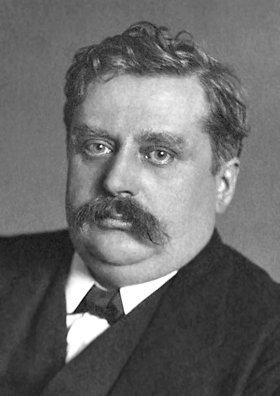
\includegraphics[width=\linewidth]{images/book3/werner.jpg}
\end{minipage}\hfill
\begin{minipage}[t]{0.74\linewidth}
\vspace{0pt}
Alfred Werner propuso en 1893 que un metal tiene, además de su valencia, un
número de coordinación de grupos sujetos directamente a su alrededor, y que el cobalto(III) sujeta
seis en los vértices de un octaedro. Predijo después cuántos isómeros debía tener cada
fórmula y pasó veinte años preparándolos; en 1911 resolvió un complejo de
cobalto en sus dos enantiómeros, demostrando que la quiralidad no exige un
átomo de carbono. Recibió el Premio Nobel de Química en 1913. (Retrato, Les Prix
Nobel, 1914, dominio público, Wikimedia Commons.)
\end{minipage}
\end{history}

\section{Ejercicios}

\begin{exercise}[$\star$]\label{exo:b2:coordination-complexes:1}
Dese la configuración $d^n$ de \ce{Ti^3+}, \ce{V^3+}, \ce{Cr^3+}, \ce{Mn^2+}, \ce{Fe^3+},
\ce{Co^2+}, \ce{Ni^2+} y \ce{Zn^2+}.
\end{exercise}

\begin{exercise}[$\star$]\label{exo:b2:coordination-complexes:2}
Dese la \omterm{def:b2:coordination-complexes:denticity}{denticidad} del agua, la etano-1,2-diamina, el ion etanodioato, el edta y el
ion tiocianato, y dígase cuál es ambidentado.
\end{exercise}

\begin{exercise}[$\star$]\label{exo:b2:coordination-complexes:3}
Nómbrense \ce{[Cu(NH3)4]SO4}, \ce{K3[Fe(CN)6]}, \ce{[CoCl2(NH3)4]Cl} y
\ce{[Ni(CO)4]}.
\end{exercise}

\begin{exercise}[$\star$]\label{exo:b2:coordination-complexes:4}
Prevéase la geometría de \ce{[Ag(NH3)2]+}, \ce{[CoCl4]^2-}, \ce{[PtCl4]^2-} y
\ce{[Fe(H2O)6]^2+}.
\end{exercise}

\begin{exercise}[$\star\star$]\label{exo:b2:coordination-complexes:5}
¿Cuántos isómeros tiene el \ce{[PtCl2(NH3)2]} plano-cuadrado? Dibújense. (Uno de ellos,
el cisplatino, es un fármaco antitumoral.)
\end{exercise}

\begin{exercise}[$\star\star$]\label{exo:b2:coordination-complexes:6}
Cuéntense los electrones de valencia de \ce{Cr(CO)6}, \ce{Fe(CO)5}, \ce{Ni(CO)4},
\ce{V(CO)6} y \ce{Mn2(CO)10}. ¿Cuál incumple la regla, y cómo se comporta?
\end{exercise}

\begin{exercise}[$\star\star$]\label{exo:b2:coordination-complexes:7}
Cuéntense los electrones de valencia del ferroceno y del cobaltoceno \ce{Co(C5H5)2}. ¿Cuál se
oxida con facilidad, y a qué?
\end{exercise}

\begin{exercise}[$\star\star$]\label{exo:b2:coordination-complexes:8}
El complejo de níquel(II) con el edta tiene $\log_{10}K = 20.5$, muy por encima del de los complejos en
los que el níquel se une a seis dadores de nitrógeno u oxígeno independientes. Explíquese este efecto quelato
en función del número de partículas liberadas cuando el quelato sustituye a seis moléculas
de agua.
% ledger: logb:Ni-edta
\end{exercise}

\begin{exercise}[$\star\star$]\label{exo:b2:coordination-complexes:9}
Dibújense los dos \omterm{def:b2:coordination-complexes:isomers}{isómeros de enlace} de \ce{[Co(NO2)(NH3)5]^2+}.
\end{exercise}

\begin{exercise}[$\star\star\star$]\label{exo:b2:coordination-complexes:10}
¿Cuántos estereoisómeros tiene \ce{[CoCl2(en)2]+}? ¿Cuáles son quirales?
\end{exercise}

\begin{exercise}[$\star\star\star$]\label{exo:b2:coordination-complexes:11}
Para $\mathrm{MA_4B_2}$, cuéntense los isómeros que predicen un hexágono plano y un prisma
trigonal de seis ligandos, y explíquese cómo el número de isómeros hallado permite decidir entre las
geometrías.
\end{exercise}

\begin{exercise}[$\star\star\star$]\label{exo:b2:coordination-complexes:12}
Cuéntense los electrones de valencia de \ce{[RhCl(PPh3)3]} y de \ce{[IrH(CO)(PPh3)3]}
(\ce{PPh3}, dador de dos electrones; \ce{H-}, como hidruro). ¿Cuál podría admitir dos
ligandos más?
\end{exercise}

\section{Problema: las amminas de cobalto de Werner}

\begin{problem}[{Problema de fin de semana --- cuatro amminas de cloruro de cobalto(III) y el cloruro
que liberan, sus fórmulas con corchetes, los dos isómeros de la tetraammina y lo que
demuestran sobre la geometría, y la actividad óptica de un tris-quelato}]
\label{pb:b2:coordination-complexes:1}
Datos: cuatro compuestos, A \ce{CoCl3.6NH3} (amarillo anaranjado), B \ce{CoCl3.5NH3}
(púrpura), C y D \ce{CoCl3.4NH3} (verde y violeta). Con nitrato de plata en exceso,
un mol de A precipita 3 mol de \ce{AgCl}, B 2 mol, y C y D 1 mol cada uno. Las conductividades
molares indican 4, 3, 2 y 2 iones por unidad fórmula.

\medskip
\noindent\textbf{Parte I --- Cloruro e iones.}
\begin{enumerate}
  \item ¿Qué cloruros reaccionan de inmediato con los iones plata?
  \item ¿Cuántos cloruros están unidos al cobalto en cada compuesto?
  \item Compruébense los números de iones con las conductividades.
  \item ¿Cuál es el número de oxidación del cobalto en los cuatro?
  \item ¿Cuál es su configuración $d^n$?
  \item ¿Cuántos ligandos en total sujeta el cobalto en cada compuesto?
\end{enumerate}

\medskip
\noindent\textbf{Parte II --- Fórmulas y nombres.}
\begin{enumerate}[resume]
  \item Escríbanse A, B, C y D con corchetes.
  \item Nómbrense A y B.
  \item Nómbrese el catión de C y D.
  \item ¿Qué tipo de isómeros son C y D?
  \item ¿Qué sería un compuesto \ce{CoCl3.3NH3}, y cuántos iones daría?
  \item ¿Cuántos isómeros tendría ese compuesto en un octaedro?
\end{enumerate}

\medskip
\noindent\textbf{Parte III --- La geometría.}
\begin{enumerate}[resume]
  \item Dibújense el \ce{[CoCl2(NH3)4]+} cis y el trans en un octaedro.
  \item Cuéntense los isómeros de \ce{[CoCl2(NH3)4]+} predichos para seis ligandos en los
        vértices de un hexágono plano.
  \item Cuéntense los predichos para un prisma trigonal.
  \item Werner nunca encontró más de dos. ¿Qué demuestra esto?
  \item ¿Es completa la demostración? ¿Qué habría significado un tercer isómero?
  \item ¿Cuál de C y D es el cis, sabiendo que el isómero cis puede convertirse en un
        quelato con etanodioato y el trans no?
\end{enumerate}

\medskip
\noindent\textbf{Parte IV --- Actividad óptica.}
\begin{enumerate}[resume]
  \item Dibújese \ce{[Co(en)3]^3+}.
  \item ¿Tiene un plano de simetría? ¿Un centro de inversión?
  \item ¿Cuántos estereoisómeros tiene?
  \item ¿Qué demuestra la resolución de un catión así en enantiómeros?
  \item ¿Es quiral \ce{[CoCl2(en)2]+} en su forma cis? ¿Y en su forma trans?
  \item ¿Por qué fue importante que Werner resolviera un complejo que no contenía carbono en absoluto?
  \item Indíquese el número de isómeros de \ce{[CoCl2(NH3)4]+} predicho por el octaedro,
        y por el hexágono plano y el prisma trigonal.
\end{enumerate}
\end{problem}
